\section{Global planning}
\label{sec:planning}

{\sc table}~\ref{table:planning} presents an overview of the main development achievements of the internship, per month. Many smaller tasks have been omitted, as well as the meetings, demonstrations and brainstorming sessions that were also an important part of the planning.

\bgroup
	\def\arraystretch{1.5}
		\begin{table}[H]
		\centering
			\begin{tabular}{|l|l|}
			\hline
			\textbf{March} & \begin{tabular}[c]{@{}l@{}}Setup and tool discovery\\ Lots of small tasks (copywriting, debugging, emails improvement...)\\ Addition of scrolling button in activity feed \\ Privacy statement update\\ Creation of User terms page\end{tabular} \\ \hline
			\textbf{April} & \begin{tabular}[c]{@{}l@{}}Creation of Unlock your city email\\ Account deletion modal improvement\\ UI components building (Label, Alert...)\\ Course page UI implementation, with inline editing\end{tabular} \\ \hline
			\textbf{May} & \begin{tabular}[c]{@{}l@{}}Implementation of reviewing process for teachers\\ Handling non-existing pages and URLs\\ Global public/private layout refactoring\\ Mobile menu fixing (close on outside click)\end{tabular} \\ \hline
			\textbf{June} & \begin{tabular}[c]{@{}l@{}}Wireframing for matchmaking flow\\ UI components building (date and time pickers)\\ Overall navigation refactoring\\ Analytics addition to new pages\end{tabular} \\ \hline
			\textbf{July} & \begin{tabular}[c]{@{}l@{}}New teachers landing page creation\\ SEO improvement for /courses page\\ Booking flow with payment UI building\end{tabular} \\ \hline
			\textbf{August} & \begin{tabular}[c]{@{}l@{}}Administrator UI implementation\\ Temporary sign-up flow addition to new teachers page\\ Modal UI component refactoring\\ Find teacher flow UI building\end{tabular} \\ \hline
			\end{tabular}
		\label{table:planning}
		\end{table}
\egroup

\newpage

\section{A course published on Konnektid's website (desktop version)}
\label{sec:courseDesktop}

\begin{figure}[H]
    \centering
    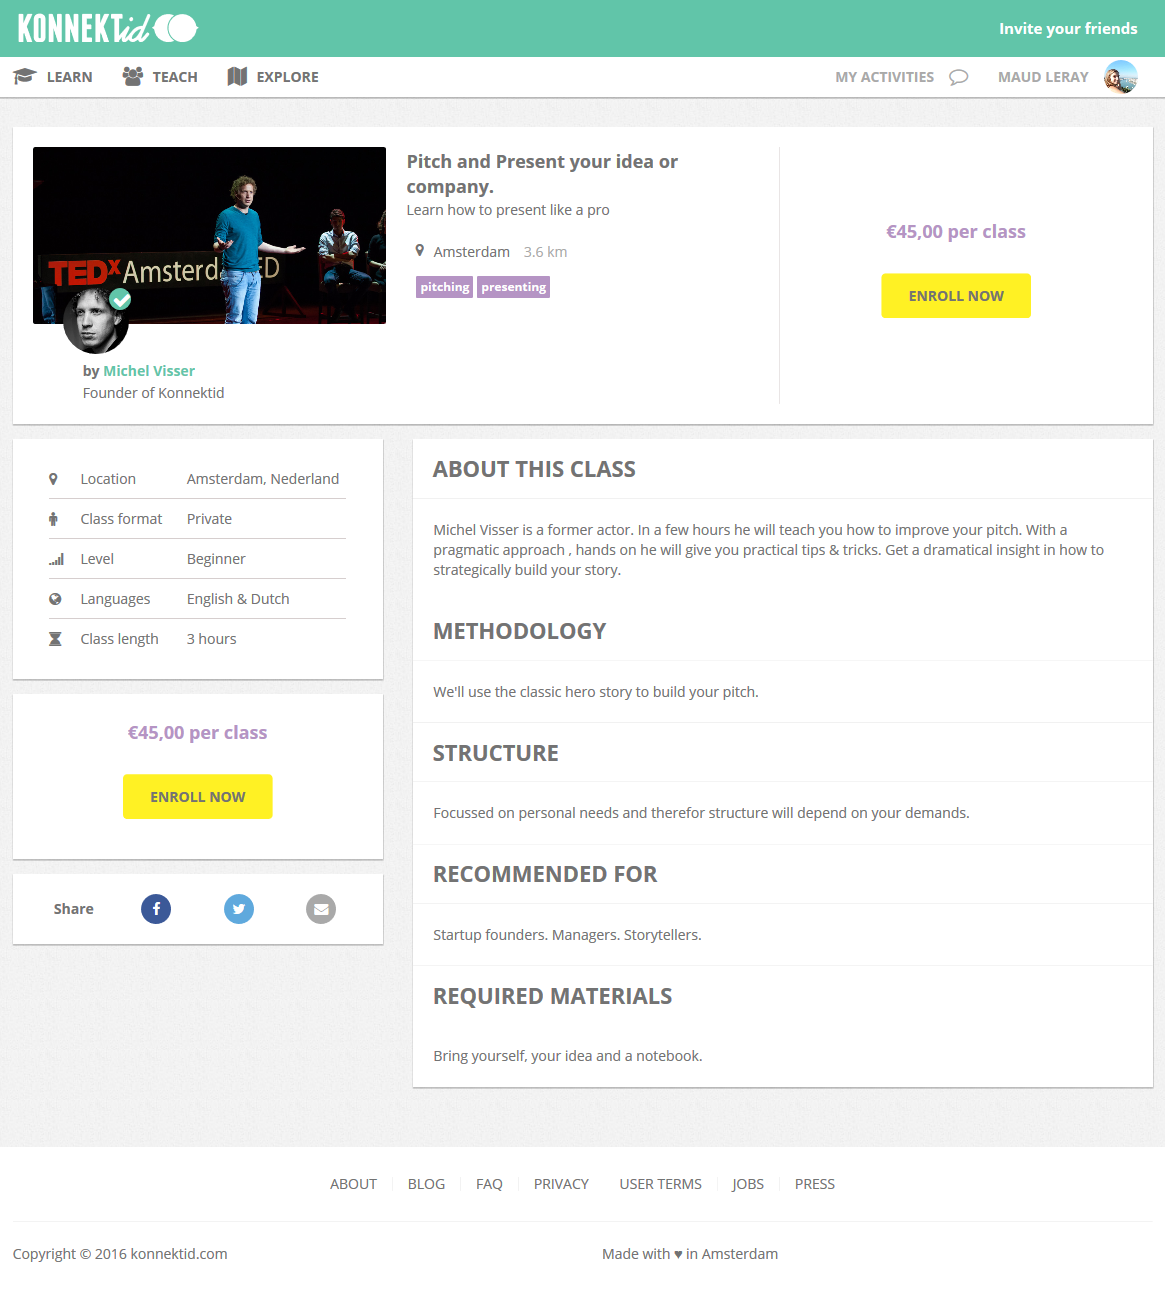
\includegraphics[scale=0.6]{figure/coursePage.png}
\end{figure}

\newpage

\section{Refactored teachers landing page (desktop version)}
\label{sec:teachersPage}

\begin{figure}[H]
    \centering
    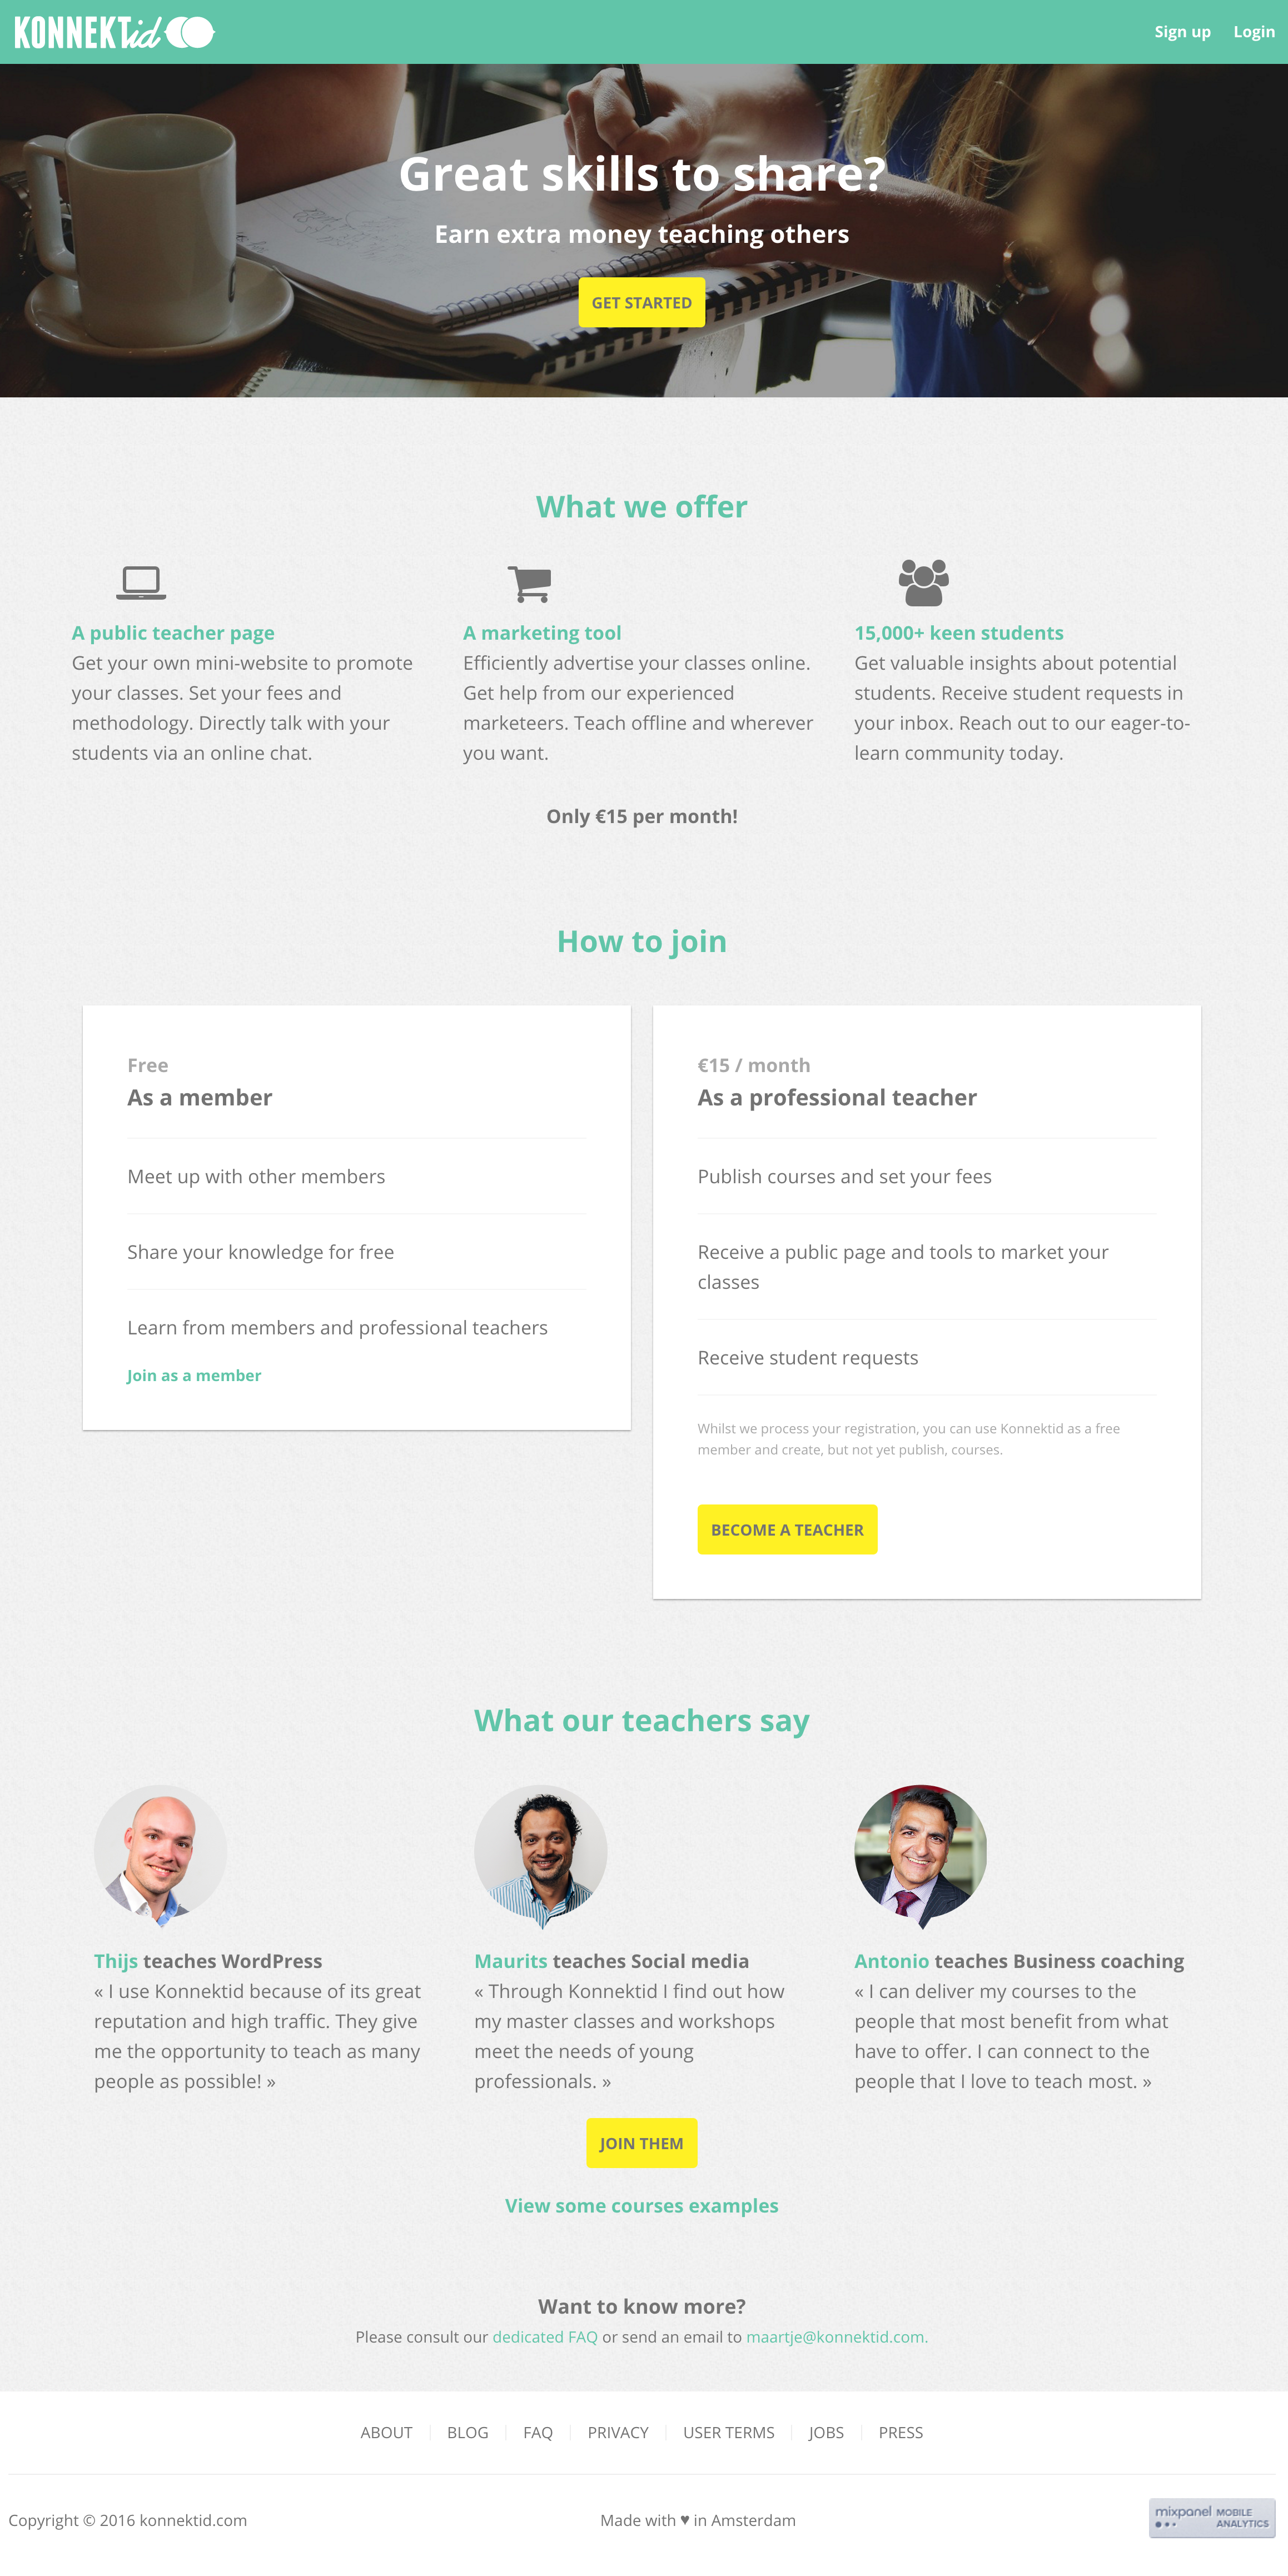
\includegraphics[scale=0.2]{figure/teachersPage.png}
\end{figure}

\newpage

\section{Homepage for the new market place (desktop version)}
\label{sec:newHome}

\begin{figure}[H]
    \centering
    \includegraphics[scale=0.1]{figure/newHome.png}
\end{figure}
